\documentclass[12pt]{beamer}
\usepackage[utf8]{inputenc}
\usepackage[T2A]{fontenc}
\usepackage[russian]{babel}
\usepackage{amsmath, amssymb, amsfonts}
\usepackage{graphicx}
\usepackage{xcolor}
\usepackage{hyperref}
\usepackage{listings}

\usetheme{Madrid}
\setbeamertemplate{caption}[numbered]
\graphicspath{{img/}}

\bibliographystyle{plain}

\title{Анализ и применение многофакторных моделей динамики лекарственных веществ в медицинских исследованиях}
\author{Лазар В. И.}
\date{\today}

\begin{document}

\begin{frame}
	\titlepage
\end{frame}

\begin{frame}{Содержание}
	\tableofcontents
\end{frame}

\section{Введение}
\begin{frame}{Введение}
	\textbf{Фармакокинетика (ФК)} – это наука, описывающая всасывание, распределение, метаболизм и выведение (ADME) лекарственных средств.

	\textbf{Ключевые факторы:}
	\begin{itemize}
		\item Физиологические и биохимические параметры
		\item Генетические особенности
		\item Внешние факторы (сопутствующее лечение, образ жизни)
	\end{itemize}

	\textbf{Проблемы анализа данных:}
	\begin{enumerate}
		\item Малые выборки
		\item Неоднородность данных во времени
		\item Высокий уровень шума в данных
		\item Наличие выбросов
	\end{enumerate}
\end{frame}

\section{Постановка задачи}
\begin{frame}{Постановка задачи}
	\textbf{Цель работы:} разработка модифицированной \textbf{PBFTPK}-модели для учета сложных траекторий концентрации лекарства в организме.

	\textbf{Требования:}
	\begin{itemize}
		\item Учет неоднократных изменений концентрации
		\item Устойчивость к шуму и выбросам
		\item Физическая интерпретируемость
		\item Работа с малыми выборками
	\end{itemize}
\end{frame}

\section{Описание данных}
\begin{frame}{Описание данных}
	\textbf{Исходные данные:} синтетические временные ряды, имитирующие реальные фармакокинетические исследования.

	\textbf{Особенности:}
	\begin{itemize}
		\item Неоднородность временных рядов
		\item Отсутствие нормализации данных
		\item Сложные формы кривых концентрации
	\end{itemize}

	\begin{center}
		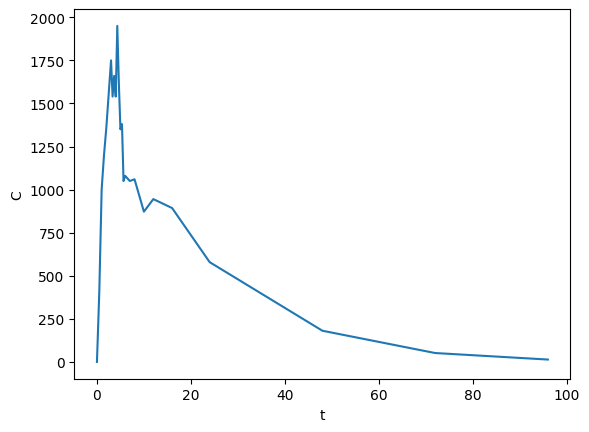
\includegraphics[width=0.45\linewidth]{sample.png}
	\end{center}
\end{frame}

\section{Описание моделей}
\begin{frame}{PBFTPK-модель}
	\textbf{Обозначения:}
	\begin{itemize}
		\item $C(t)$ – концентрация лекарства
		\item $F$ – биодоступность
		\item $D$ – введённая доза
		\item $V_d$ – объём распределения
		\item $k_a, k_{el}$ – коэффициенты всасывания и элиминации
	\end{itemize}

	\textbf{Формула модели:}
	\[ C(t) = \frac{FD k_a}{V_d (k_a - k_{el})} (e^{-k_{el}t} - e^{-k_a t}) \]
\end{frame}

\begin{frame}{Функции потерь}
	\textbf{Используемая функция потерь:}
	\[ L_{\lambda} = \frac{1}{N} \sum_{i=1}^{N} l_{\lambda}(C, \hat{C}, t_i) \]

	\textbf{Где:}
	\[ l_{\lambda}(C, \hat{C}, t) = (C(t) - \hat{C}(t)) ^ 2 \cdot \begin{cases}
			1, t \leq \tau \\
			\lambda, t > \tau
		\end{cases} \]

	\textbf{Регулировка ошибки:}
	\begin{itemize}
		\item $\lambda < 1$ – точность оценки на этапе абсорбции важнее
		\item $\lambda > 1$ – точность оценки на этапе выведения важнее
		\item $\lambda = 1$ – стандартная среднеквадратичная ошибка (MSE)
	\end{itemize}
\end{frame}

\section{Полученные результаты}
\begin{frame}{Сравнение моделей}
	\begin{minipage}{0.45\linewidth}
		\centering
		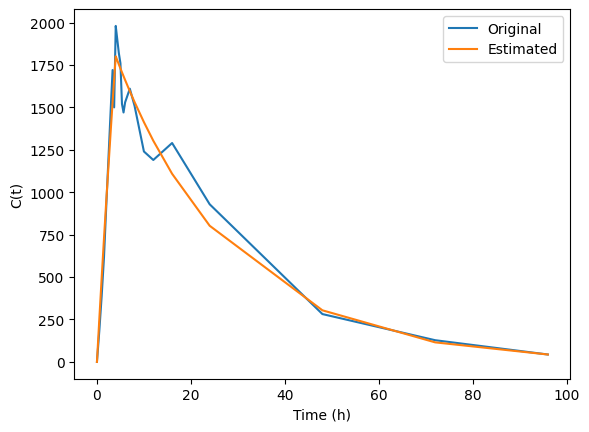
\includegraphics[width=\linewidth]{results/basic_1.png}
		% \caption{PBFTPK (Пример 1)}
		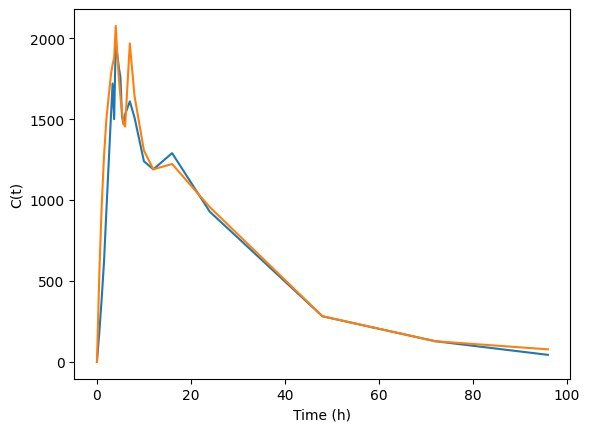
\includegraphics[width=\linewidth]{results/1.jpg}
		% \caption{EPBFTPK (Пример 1)}
	\end{minipage}
	\begin{minipage}{0.45\linewidth}
		\centering
		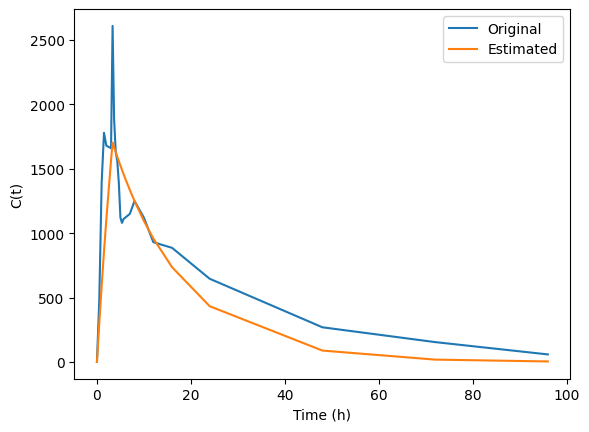
\includegraphics[width=\linewidth]{results/basic_2.png}
		% \caption{PBFTPK (Пример 2)}
		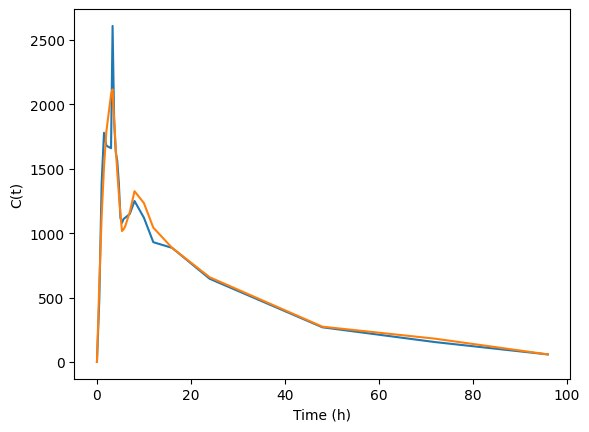
\includegraphics[width=\linewidth]{results/2.jpg}
		% \caption{EPBFTPK (Пример 2)}
	\end{minipage}
\end{frame}

\begin{frame}{Дополнительные примеры}
	\begin{minipage}{0.45\linewidth}
		\centering
		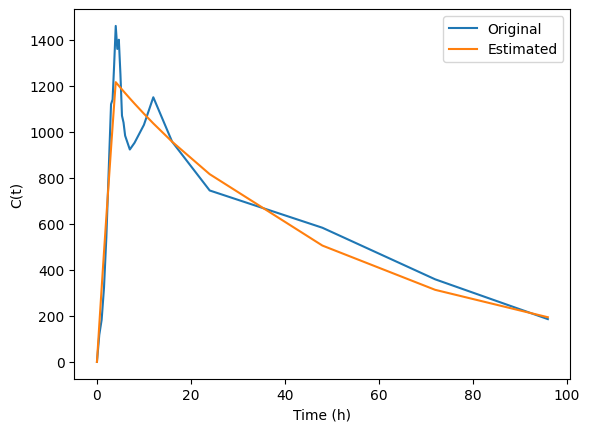
\includegraphics[width=\linewidth]{results/basic_3.png}
		% \caption{PBFTPK (Пример 3)}
		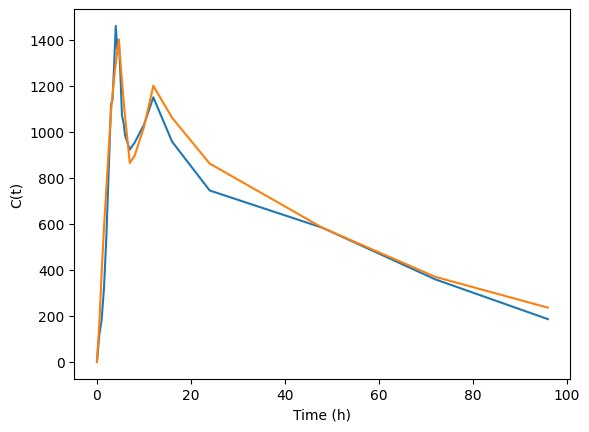
\includegraphics[width=\linewidth]{results/3.jpg}
		% \caption{EPBFTPK (Пример 3)}
	\end{minipage}
	\begin{minipage}{0.45\linewidth}
		\centering
		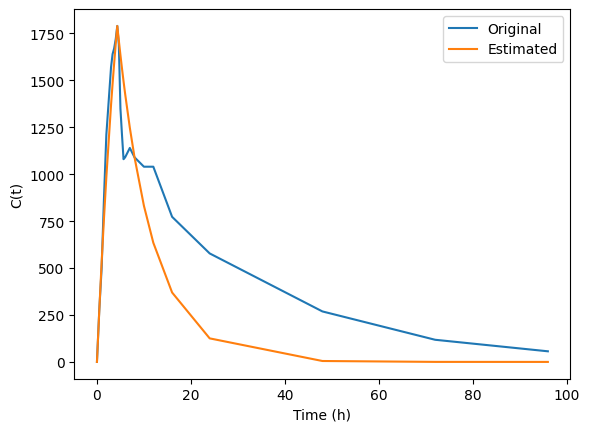
\includegraphics[width=\linewidth]{results/basic_4.png}
		% \caption{PBFTPK (Пример 4)}
		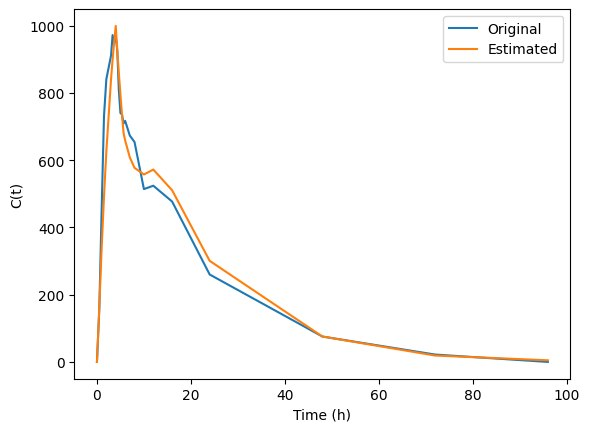
\includegraphics[width=\linewidth]{results/4.jpg}
		% \caption{EPBFTPK (Пример 4)}
	\end{minipage}
\end{frame}

\begin{frame}{Выводы}
	\textbf{Основные результаты:}
	\begin{itemize}
		\item Улучшенная EPBFTPK-модель более точно описывает траектории концентрации
		\item Учет шума, выбросов и сложных траекторий
		\item Выбор параметров модели позволяет адаптироваться к различным сценариям
	\end{itemize}
\end{frame}


\begin{frame}
	\bibliography{refs}
	\hphantom{\cite{chryssafidis}
		\cite{macheras}
		\cite{rowland}
	}
\end{frame}
\end{document}
